\section{System Design and Implementation}

\subsection{System Architecture Overview}
The TrackMyBills system adopts a client-server architecture that separates user interface concerns from computational-intensive deep learning processing. The architecture consists of two primary components: a Flutter-based mobile application for user interaction and a FastAPI-based backend service for model inference. This separation allows the system to provide responsive user experience while leveraging cloud-based processing power for the deep learning models.

The mobile application handles all user-facing functionality including image capture, preprocessing, result visualization, and local data storage. The application implements a clean architecture pattern that separates presentation, domain, and data layers, facilitating maintainable code and testable components. User interactions flow through well-defined interfaces that abstract the complexity of backend communication and data management.

The backend service provides RESTful API endpoints for model inference, implementing both base and custom Donut models for different document types. The service architecture supports concurrent request processing and includes comprehensive error handling and logging for production deployment. Model loading and inference are optimized for response time while maintaining accuracy standards required for practical expense tracking applications.

\begin{figure}[htbp]
    \centerline{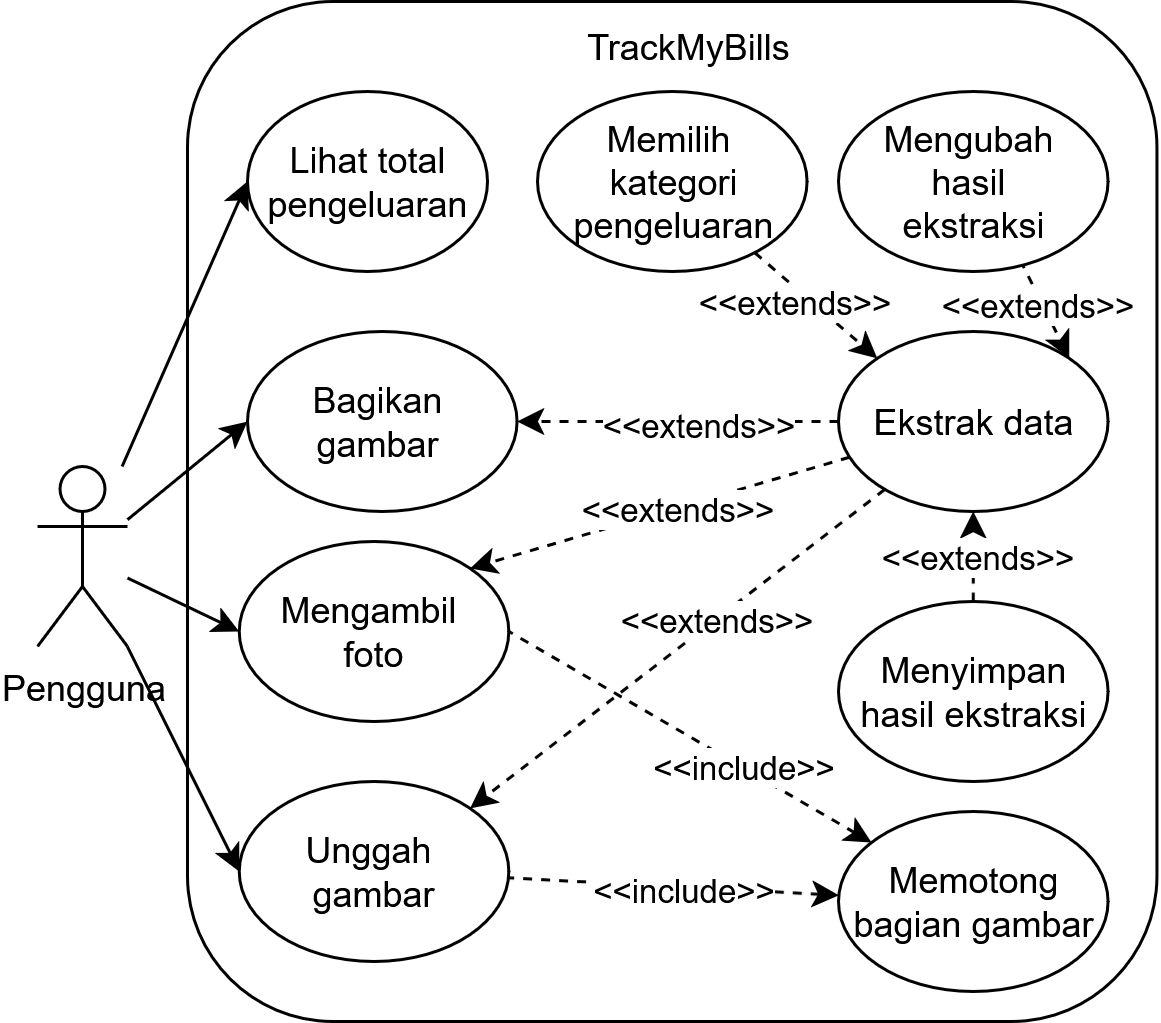
\includegraphics[width=0.45\textwidth]{images/use-case-diagram.png}}
    \caption{Use Case Diagram of TrackMyBills System}
    \label{fig:usecase}
\end{figure}

The use case diagram shown in Figure \ref{fig:usecase} illustrates the primary interactions between users and the system. Users can upload images from camera or gallery, crop images for optimal processing, initiate data extraction, review and edit extracted information, categorize transactions, and save records for future reference. Each use case is designed to minimize user effort while providing sufficient control over the extraction and categorization process.

\subsection{Mobile Application Design}
The TrackMyBills mobile application implements a user-centered design philosophy that prioritizes ease of use and visual clarity. The application workflow guides users through a streamlined process from image capture to transaction recording, minimizing the number of steps required to complete expense tracking tasks. The interface design follows Material Design principles while incorporating visual elements that appeal to Gen Z users.

The image capture and preprocessing module provides multiple input options including camera capture and gallery selection, accommodating different user preferences and scenarios. The cropping functionality allows users to focus the extraction process on relevant document areas, improving accuracy by eliminating background noise and irrelevant visual elements. The preprocessing pipeline includes automatic image enhancement and format standardization to optimize input for the deep learning models.

The data review and editing interface presents extracted information in an intuitive form layout that allows users to verify and correct any extraction errors. The interface includes intelligent form validation and suggestion features that help users complete missing information efficiently. Category selection is implemented through a user-friendly picker interface that supports both predefined categories and custom classification options.

Local data storage utilizes SQLite for offline functionality and data persistence, ensuring that user data remains accessible without network connectivity. The storage schema is designed to support future features such as expense analytics, budgeting, and data export functionality. Data synchronization capabilities are architected to support future cloud storage integration while maintaining user privacy and data ownership.

\subsection{Backend Service Architecture}
The DonutAPI backend service implements a microservices-inspired architecture that isolates model inference from other system concerns. The service exposes RESTful endpoints for document processing, supporting both synchronous and asynchronous processing modes depending on model complexity and expected processing time. The API design follows OpenAPI specifications, providing comprehensive documentation and enabling easy integration with client applications.

Model management within the backend service supports multiple Donut model instances optimized for different document types. The base model, fine-tuned on the CORD-v2 dataset, specializes in paper receipt processing and handles traditional merchant receipts with standardized layouts. The custom model, trained on the QRIS-TF dataset, focuses on digital payment documents from Indonesian financial applications including GoPay, SeaBank, Neobank, and BCA transfer receipts.

Request processing includes comprehensive input validation, image preprocessing, and result formatting to ensure consistent API behavior. Error handling mechanisms provide detailed feedback for various failure modes including invalid image formats, processing timeouts, and model inference errors. Logging and monitoring capabilities support production deployment and performance optimization.

\begin{figure}[htbp]
    \centerline{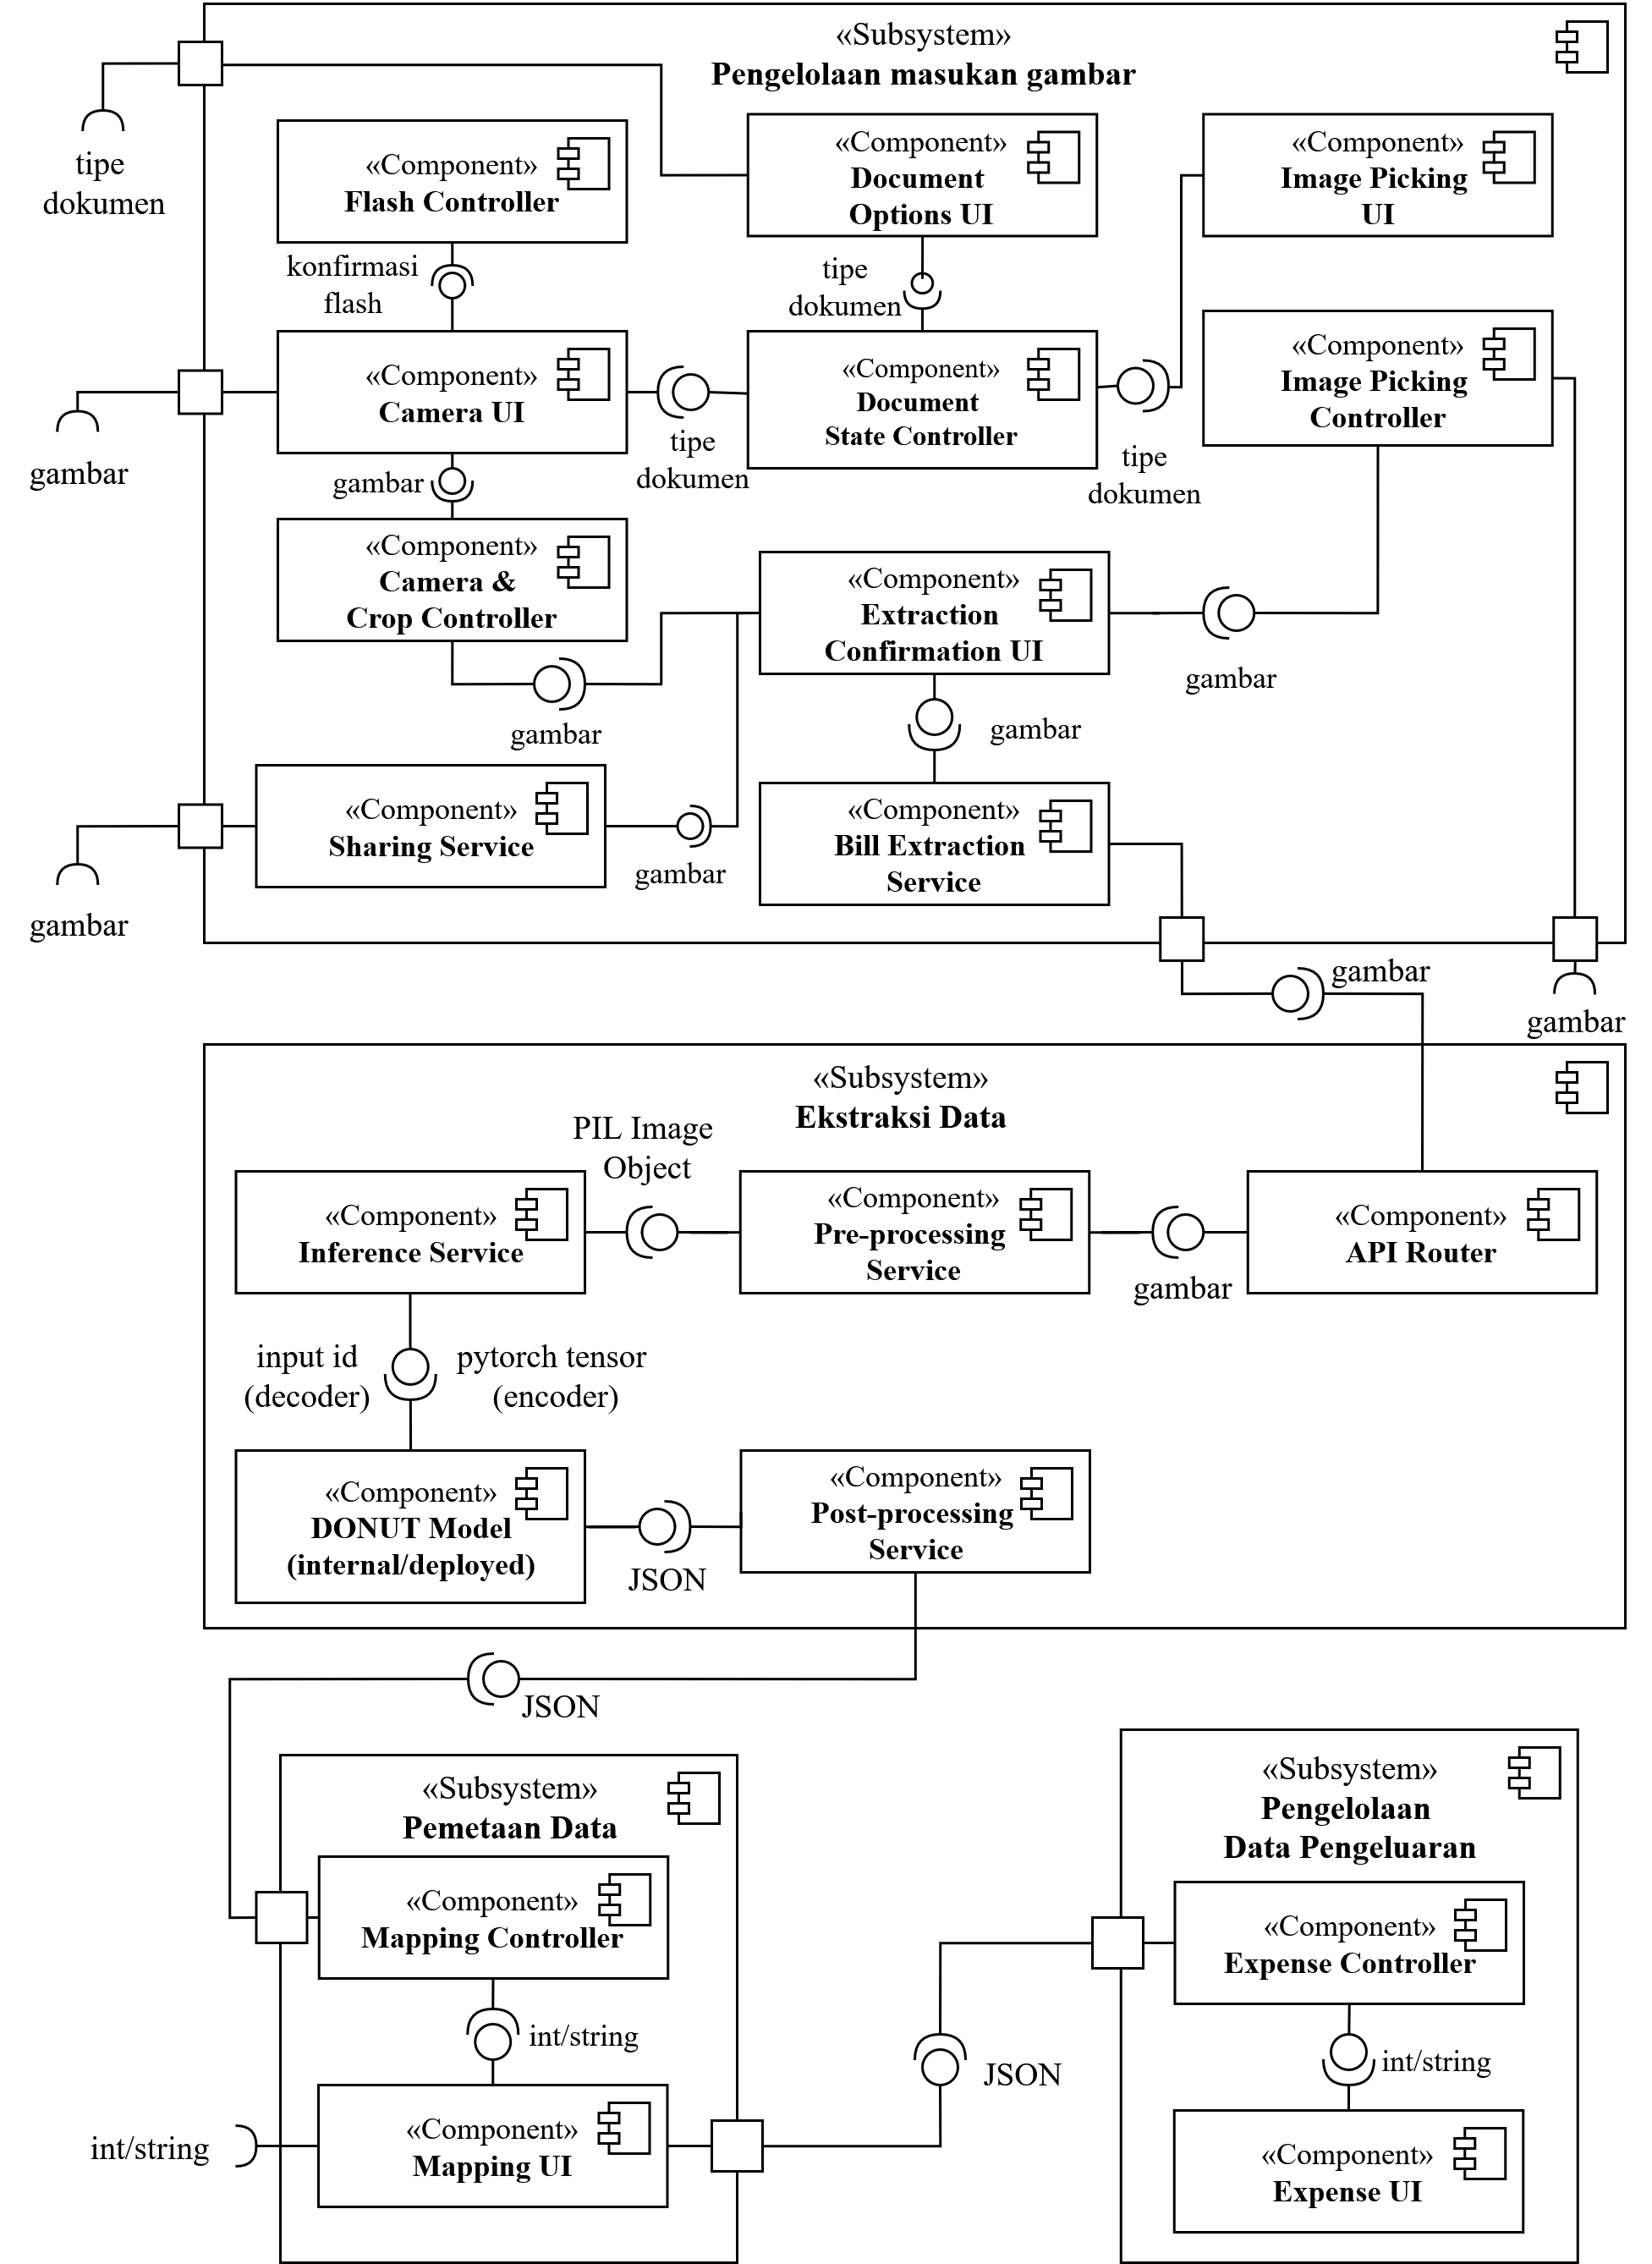
\includegraphics[width=0.45\textwidth]{images/component-diagram.png}}
    \caption{Component Diagram of the System}
    \label{fig:component}
\end{figure}

\subsection{Development Methodology}
The system development follows the Design Science Research Methodology (DSRM) framework, which provides a structured approach to developing and evaluating technology artifacts for solving identified problems. The methodology encompasses six phases: problem identification and motivation, objective definition for solution, design and development, demonstration, evaluation, and communication.

\begin{figure}[htbp]
    \centerline{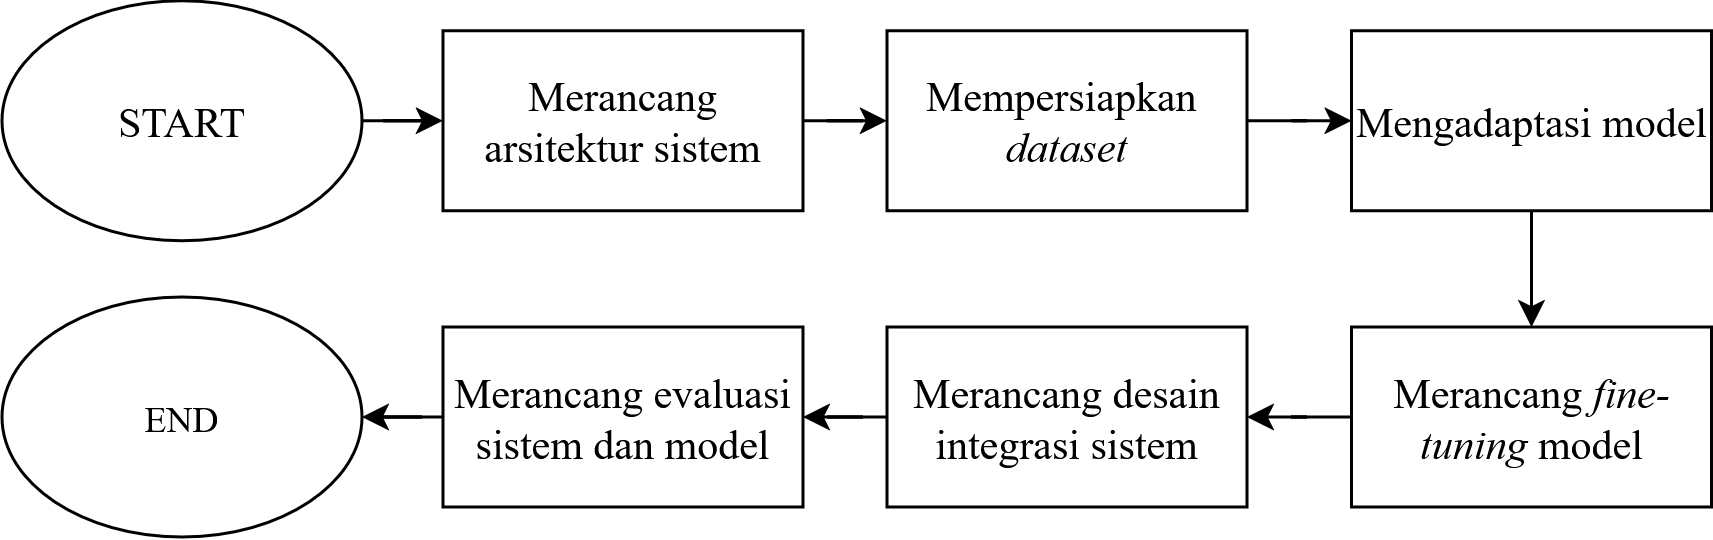
\includegraphics[width=0.45\textwidth]{images/design-flow.png}}
    \caption{Planned Development Flow}
    \label{fig:devflow}
\end{figure}

The development flow illustrated in Figure \ref{fig:devflow} begins with comprehensive problem analysis focusing on Gen Z expense tracking challenges in the QRIS payment ecosystem. Objective definition establishes clear success criteria including accuracy thresholds for data extraction, usability benchmarks for user experience, and performance requirements for mobile deployment.

The design and development phase encompasses both data science and software engineering activities. Dataset preparation involves collecting and annotating payment documents from various sources, ensuring representation of real-world format diversity. Model development includes fine-tuning pre-trained Donut models on domain-specific datasets, with careful attention to overfitting prevention and generalization performance.

\subsection{Dataset Preparation and Model Training}
The research utilizes two complementary datasets to address different document processing requirements. The CORD-v2 dataset provides a foundation for general receipt processing, containing 1,000 annotated images of paper receipts with structured ground truth labels. This publicly available dataset enables comparison with existing research while providing sufficient data for transfer learning.

The custom QRIS-TF dataset addresses the specific requirements of Indonesian digital payment processing, containing 200 carefully curated images representing payment receipts from major Indonesian financial applications. Dataset creation involved systematic collection of QRIS payment receipts, bank transfer confirmations, and digital wallet transactions across different applications and merchant types. Annotation follows a structured schema that captures essential transaction information including amounts, timestamps, merchant identifiers, and transaction types.

Data preprocessing includes image normalization, format standardization, and augmentation techniques to improve model robustness. Augmentation strategies include rotation, scaling, and lighting variation to simulate real-world capture conditions. Training procedures implement early stopping and learning rate scheduling to optimize convergence while preventing overfitting on the relatively small custom dataset.

\begin{figure}[htbp]
    \centerline{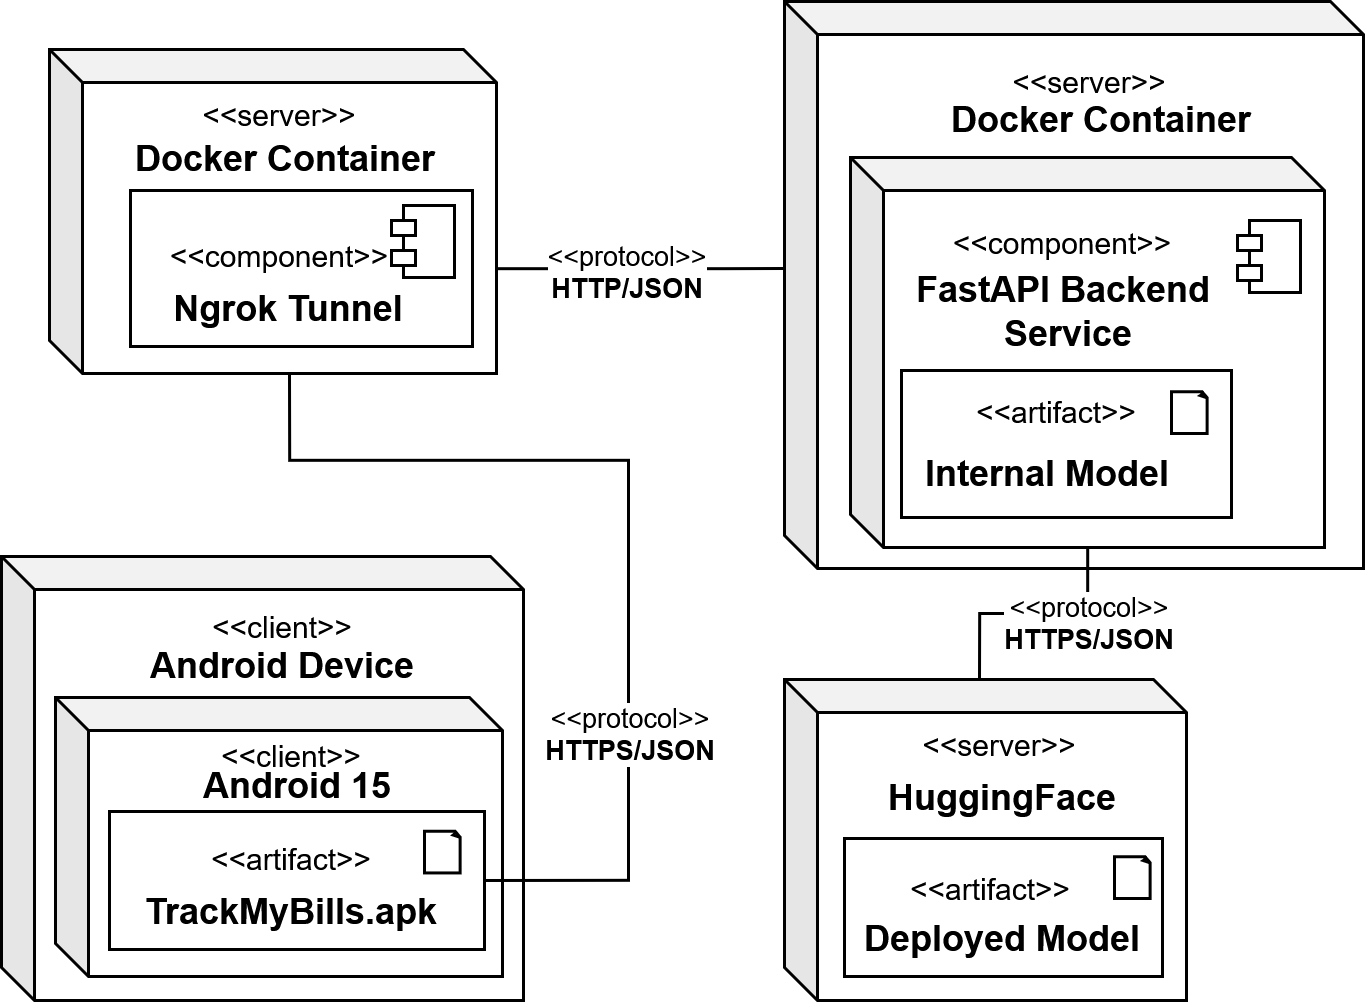
\includegraphics[width=0.45\textwidth]{images/deployment-diagram.png}}
    \caption{Deployment Architecture}
    \label{fig:deployment}
\end{figure}

The deployment architecture shown in Figure \ref{fig:deployment} illustrates the production environment configuration. The mobile application communicates with the backend service through HTTPS REST API calls, ensuring secure data transmission. The backend service is containerized using Docker for consistent deployment across different cloud platforms. Model artifacts are versioned and managed separately to enable independent model updates without service disruption.